\documentclass[twoside]{book}

% Packages required by doxygen
\usepackage{fixltx2e}
\usepackage{calc}
\usepackage{doxygen}
\usepackage[export]{adjustbox} % also loads graphicx
\usepackage{graphicx}
\usepackage[utf8]{inputenc}
\usepackage{makeidx}
\usepackage{multicol}
\usepackage{multirow}
\PassOptionsToPackage{warn}{textcomp}
\usepackage{textcomp}
\usepackage[nointegrals]{wasysym}
\usepackage[table]{xcolor}

% NLS support packages
\usepackage[catalan]{babel}

% Font selection
\usepackage[T1]{fontenc}
\usepackage[scaled=.90]{helvet}
\usepackage{courier}
\usepackage{amssymb}
\usepackage{sectsty}
\renewcommand{\familydefault}{\sfdefault}
\allsectionsfont{%
  \fontseries{bc}\selectfont%
  \color{darkgray}%
}
\renewcommand{\DoxyLabelFont}{%
  \fontseries{bc}\selectfont%
  \color{darkgray}%
}
\newcommand{\+}{\discretionary{\mbox{\scriptsize$\hookleftarrow$}}{}{}}

% Page & text layout
\usepackage{geometry}
\geometry{%
  a4paper,%
  top=2.5cm,%
  bottom=2.5cm,%
  left=2.5cm,%
  right=2.5cm%
}
\tolerance=750
\hfuzz=15pt
\hbadness=750
\setlength{\emergencystretch}{15pt}
\setlength{\parindent}{0cm}
\setlength{\parskip}{3ex plus 2ex minus 2ex}
\makeatletter
\renewcommand{\paragraph}{%
  \@startsection{paragraph}{4}{0ex}{-1.0ex}{1.0ex}{%
    \normalfont\normalsize\bfseries\SS@parafont%
  }%
}
\renewcommand{\subparagraph}{%
  \@startsection{subparagraph}{5}{0ex}{-1.0ex}{1.0ex}{%
    \normalfont\normalsize\bfseries\SS@subparafont%
  }%
}
\makeatother

% Headers & footers
\usepackage{fancyhdr}
\pagestyle{fancyplain}
\fancyhead[LE]{\fancyplain{}{\bfseries\thepage}}
\fancyhead[CE]{\fancyplain{}{}}
\fancyhead[RE]{\fancyplain{}{\bfseries\leftmark}}
\fancyhead[LO]{\fancyplain{}{\bfseries\rightmark}}
\fancyhead[CO]{\fancyplain{}{}}
\fancyhead[RO]{\fancyplain{}{\bfseries\thepage}}
\fancyfoot[LE]{\fancyplain{}{}}
\fancyfoot[CE]{\fancyplain{}{}}
\fancyfoot[RE]{\fancyplain{}{\bfseries\scriptsize Generat per Doxygen }}
\fancyfoot[LO]{\fancyplain{}{\bfseries\scriptsize Generat per Doxygen }}
\fancyfoot[CO]{\fancyplain{}{}}
\fancyfoot[RO]{\fancyplain{}{}}
\renewcommand{\footrulewidth}{0.4pt}
\renewcommand{\chaptermark}[1]{%
  \markboth{#1}{}%
}
\renewcommand{\sectionmark}[1]{%
  \markright{\thesection\ #1}%
}

% Indices & bibliography
\usepackage{natbib}
\usepackage[titles]{tocloft}
\setcounter{tocdepth}{3}
\setcounter{secnumdepth}{5}
\makeindex

% Hyperlinks (required, but should be loaded last)
\usepackage{ifpdf}
\ifpdf
  \usepackage[pdftex,pagebackref=true]{hyperref}
\else
  \usepackage[ps2pdf,pagebackref=true]{hyperref}
\fi
\hypersetup{%
  colorlinks=true,%
  linkcolor=blue,%
  citecolor=blue,%
  unicode%
}

% Custom commands
\newcommand{\clearemptydoublepage}{%
  \newpage{\pagestyle{empty}\cleardoublepage}%
}

\usepackage{caption}
\captionsetup{labelsep=space,justification=centering,font={bf},singlelinecheck=off,skip=4pt,position=top}

%===== C O N T E N T S =====

\begin{document}

% Titlepage & ToC
\hypersetup{pageanchor=false,
             bookmarksnumbered=true,
             pdfencoding=unicode
            }
\pagenumbering{alph}
\begin{titlepage}
\vspace*{7cm}
\begin{center}%
{\Large X90633 Control -\/ Torn 1 (Primavera 2015) \\[1ex]\large Ricard Guixaró Trancho }\\
\vspace*{1cm}
{\large Generat per Doxygen 1.8.13}\\
\end{center}
\end{titlepage}
\clearemptydoublepage
\pagenumbering{roman}
\tableofcontents
\clearemptydoublepage
\pagenumbering{arabic}
\hypersetup{pageanchor=true}

%--- Begin generated contents ---
\chapter{Exemple de disseny modular\+: X90633 Control -\/ Torn 1 (Primavera 2015).}
\label{index}\hypertarget{index}{}En esta practica se construye un programa modular que ofrece un menú de opciones para gestionar un almacen. Se introducen las clases {\itshape \hyperlink{class_cjt__productos}{Cjt\+\_\+productos}}, {\itshape \hyperlink{class_sala}{Sala}}, {\itshape \hyperlink{class_cjt__salas}{Cjt\+\_\+salas}} y {\itshape \hyperlink{class_almacen}{Almacen}}. 
\chapter{Índex de Classes}
\section{Llista de Classes}
Aquestes són les classes, estructures, unions i interfícies acompanyades amb breus descripcions\+:\begin{DoxyCompactList}
\item\contentsline{section}{\hyperlink{class_cjt__estudiants}{Cjt\+\_\+estudiants} \\*Representa un conjunt d\textquotesingle{}estudiants ordenat per D\+NI }{\pageref{class_cjt__estudiants}}{}
\item\contentsline{section}{\hyperlink{class_estudiant}{Estudiant} \\*Representa un estudiant amb D\+NI i la possibilitat de tenir nota }{\pageref{class_estudiant}}{}
\end{DoxyCompactList}

\chapter{Índex de Fitxers}
\section{Llista dels Fitxers}
Aquesta és la llista de tots els fitxers acompanyats amb breus descripcions\+:\begin{DoxyCompactList}
\item\contentsline{section}{\hyperlink{_bin_tree_8hh}{Bin\+Tree.\+hh} }{\pageref{_bin_tree_8hh}}{}
\item\contentsline{section}{\hyperlink{_cjt___clusters_8cc}{Cjt\+\_\+\+Clusters.\+cc} \\*Implementació de la classe \hyperlink{class_cjt___clusters}{Cjt\+\_\+\+Clusters} }{\pageref{_cjt___clusters_8cc}}{}
\item\contentsline{section}{\hyperlink{_cjt___clusters_8hh}{Cjt\+\_\+\+Clusters.\+hh} \\*Especificació de la classe \hyperlink{class_cjt___clusters}{Cjt\+\_\+\+Clusters} }{\pageref{_cjt___clusters_8hh}}{}
\item\contentsline{section}{\hyperlink{_cjt___especies_8cc}{Cjt\+\_\+\+Especies.\+cc} \\*Implementació de la classe \hyperlink{class_cjt___especies}{Cjt\+\_\+\+Especies} }{\pageref{_cjt___especies_8cc}}{}
\item\contentsline{section}{\hyperlink{_cjt___especies_8hh}{Cjt\+\_\+\+Especies.\+hh} \\*Especificació de la classe \hyperlink{class_cjt___especies}{Cjt\+\_\+\+Especies} }{\pageref{_cjt___especies_8hh}}{}
\item\contentsline{section}{\hyperlink{_cluster_8cc}{Cluster.\+cc} \\*Implementació de la classe \hyperlink{class_cluster}{Cluster} }{\pageref{_cluster_8cc}}{}
\item\contentsline{section}{\hyperlink{_cluster_8hh}{Cluster.\+hh} \\*Especificació de la classe \hyperlink{class_cluster}{Cluster} }{\pageref{_cluster_8hh}}{}
\item\contentsline{section}{\hyperlink{_especie_8cc}{Especie.\+cc} \\*Implementació de la classe \hyperlink{class_especie}{Especie} }{\pageref{_especie_8cc}}{}
\item\contentsline{section}{\hyperlink{_especie_8hh}{Especie.\+hh} \\*Especificació de la classe \hyperlink{class_especie}{Especie} }{\pageref{_especie_8hh}}{}
\item\contentsline{section}{\hyperlink{program_8cc}{program.\+cc} \\*Programa principal de la pràctica }{\pageref{program_8cc}}{}
\end{DoxyCompactList}

\chapter{Documentació de les Classes}
\hypertarget{class_cjt__estudiants}{}\section{Referència de la Classe Cjt\+\_\+estudiants}
\label{class_cjt__estudiants}\index{Cjt\+\_\+estudiants@{Cjt\+\_\+estudiants}}


Representa un conjunt d\textquotesingle{}estudiants ordenat per D\+NI.  


\subsection*{Mètodes públics}
\begin{DoxyCompactItemize}
\item 
\hyperlink{class_cjt__estudiants_a31ffe72cadcf58d82c8b9f6659c56e7a}{Cjt\+\_\+estudiants} ()
\begin{DoxyCompactList}\small\item\em Creadora per defecte. \end{DoxyCompactList}\item 
void \hyperlink{class_cjt__estudiants_a4188715904e017fa15b9ad8bc63112b6}{afegir\+\_\+estudiant} (const \hyperlink{class_estudiant}{Estudiant} \&est, bool \&b)
\begin{DoxyCompactList}\small\item\em Afegir un estudiant a un conjunt. \end{DoxyCompactList}\item 
void \hyperlink{class_cjt__estudiants_a6632e0cecaa9d698cb51da07c9e58402}{esborrar\+\_\+estudiant} (int dni, bool \&b)
\begin{DoxyCompactList}\small\item\em Esborrar un estudiant d\textquotesingle{}un conjunt. \end{DoxyCompactList}\item 
int \hyperlink{class_cjt__estudiants_a87c69704a0eff48a301cfff05e6dd587}{mida} () const
\begin{DoxyCompactList}\small\item\em Mida d\textquotesingle{}un conjunt. \end{DoxyCompactList}\item 
double \hyperlink{class_cjt__estudiants_a8c8099d5080864a677743e5e1d1bbdf8}{mitjana\+\_\+estudiants\+\_\+amb\+\_\+nota} () const
\begin{DoxyCompactList}\small\item\em Consulta de la mitjana dels estudiants amb nota d\textquotesingle{}un conjunt. \end{DoxyCompactList}\item 
void \hyperlink{class_cjt__estudiants_aa24c2d4c36167b2b810ab459435b67a8}{llegir} ()
\begin{DoxyCompactList}\small\item\em Lectura d\textquotesingle{}un conjunt d\textquotesingle{}estudiants. \end{DoxyCompactList}\item 
void \hyperlink{class_cjt__estudiants_a2c25dbd33850025de3389617712f896a}{escriure} () const
\begin{DoxyCompactList}\small\item\em Escriptura d\textquotesingle{}un conjunt d\textquotesingle{}estudiants. \end{DoxyCompactList}\end{DoxyCompactItemize}
\subsection*{Mètodes Públics Estàtics}
\begin{DoxyCompactItemize}
\item 
static int \hyperlink{class_cjt__estudiants_a171fdff58b408ccbf647ab594b5eafa4}{mida\+\_\+maxima} ()
\begin{DoxyCompactList}\small\item\em Consultora de la mida màxima d\textquotesingle{}un conjunt. \end{DoxyCompactList}\end{DoxyCompactItemize}


\subsection{Descripció Detallada}
Representa un conjunt d\textquotesingle{}estudiants ordenat per D\+NI. 

Definició a la línia 18 del fitxer Cjt\+\_\+estudiants.\+hh.



\subsection{Documentació del Constructor i el Destructor}
\mbox{\Hypertarget{class_cjt__estudiants_a31ffe72cadcf58d82c8b9f6659c56e7a}\label{class_cjt__estudiants_a31ffe72cadcf58d82c8b9f6659c56e7a}} 
\index{Cjt\+\_\+estudiants@{Cjt\+\_\+estudiants}!Cjt\+\_\+estudiants@{Cjt\+\_\+estudiants}}
\index{Cjt\+\_\+estudiants@{Cjt\+\_\+estudiants}!Cjt\+\_\+estudiants@{Cjt\+\_\+estudiants}}
\subsubsection{\texorpdfstring{Cjt\+\_\+estudiants()}{Cjt\_estudiants()}}
{\footnotesize\ttfamily Cjt\+\_\+estudiants\+::\+Cjt\+\_\+estudiants (\begin{DoxyParamCaption}{ }\end{DoxyParamCaption})}



Creadora per defecte. 

\begin{DoxyPrecond}{Precondició}
{\itshape cert} 
\end{DoxyPrecond}
\begin{DoxyPostcond}{Postcondició}
Crea un conjunt d\textquotesingle{}estudiants buit 
\end{DoxyPostcond}


\subsection{Documentació de les Funcions Membre}
\mbox{\Hypertarget{class_cjt__estudiants_a4188715904e017fa15b9ad8bc63112b6}\label{class_cjt__estudiants_a4188715904e017fa15b9ad8bc63112b6}} 
\index{Cjt\+\_\+estudiants@{Cjt\+\_\+estudiants}!afegir\+\_\+estudiant@{afegir\+\_\+estudiant}}
\index{afegir\+\_\+estudiant@{afegir\+\_\+estudiant}!Cjt\+\_\+estudiants@{Cjt\+\_\+estudiants}}
\subsubsection{\texorpdfstring{afegir\+\_\+estudiant()}{afegir\_estudiant()}}
{\footnotesize\ttfamily void Cjt\+\_\+estudiants\+::afegir\+\_\+estudiant (\begin{DoxyParamCaption}\item[{const \hyperlink{class_estudiant}{Estudiant} \&}]{est,  }\item[{bool \&}]{b }\end{DoxyParamCaption})}



Afegir un estudiant a un conjunt. 

\begin{DoxyPrecond}{Precondició}
El paràmetre implícit no està ple 
\end{DoxyPrecond}
\begin{DoxyPostcond}{Postcondició}
b = indica si el p.\+i. original contè un estudiant amb el dni d\textquotesingle{}est; si b = fals, s\textquotesingle{}ha afegit l\textquotesingle{}estudiant est al paràmetre implícit 
\end{DoxyPostcond}
\mbox{\Hypertarget{class_cjt__estudiants_a6632e0cecaa9d698cb51da07c9e58402}\label{class_cjt__estudiants_a6632e0cecaa9d698cb51da07c9e58402}} 
\index{Cjt\+\_\+estudiants@{Cjt\+\_\+estudiants}!esborrar\+\_\+estudiant@{esborrar\+\_\+estudiant}}
\index{esborrar\+\_\+estudiant@{esborrar\+\_\+estudiant}!Cjt\+\_\+estudiants@{Cjt\+\_\+estudiants}}
\subsubsection{\texorpdfstring{esborrar\+\_\+estudiant()}{esborrar\_estudiant()}}
{\footnotesize\ttfamily void Cjt\+\_\+estudiants\+::esborrar\+\_\+estudiant (\begin{DoxyParamCaption}\item[{int}]{dni,  }\item[{bool \&}]{b }\end{DoxyParamCaption})}



Esborrar un estudiant d\textquotesingle{}un conjunt. 

\begin{DoxyPrecond}{Precondició}
{\itshape cert} 
\end{DoxyPrecond}
\begin{DoxyPostcond}{Postcondició}
b indica si el paràmetre implícit original tenia un estudiant amb el dni dni; si b, aquest estudiant ha quedat eliminat del paràmetre implícit 
\end{DoxyPostcond}
\mbox{\Hypertarget{class_cjt__estudiants_a87c69704a0eff48a301cfff05e6dd587}\label{class_cjt__estudiants_a87c69704a0eff48a301cfff05e6dd587}} 
\index{Cjt\+\_\+estudiants@{Cjt\+\_\+estudiants}!mida@{mida}}
\index{mida@{mida}!Cjt\+\_\+estudiants@{Cjt\+\_\+estudiants}}
\subsubsection{\texorpdfstring{mida()}{mida()}}
{\footnotesize\ttfamily int Cjt\+\_\+estudiants\+::mida (\begin{DoxyParamCaption}{ }\end{DoxyParamCaption}) const}



Mida d\textquotesingle{}un conjunt. 

\begin{DoxyPrecond}{Precondició}
{\itshape cert} 
\end{DoxyPrecond}
\begin{DoxyPostcond}{Postcondició}
El resultat és el nombre d\textquotesingle{}estudiants del paràmetre implícit 
\end{DoxyPostcond}
\mbox{\Hypertarget{class_cjt__estudiants_a171fdff58b408ccbf647ab594b5eafa4}\label{class_cjt__estudiants_a171fdff58b408ccbf647ab594b5eafa4}} 
\index{Cjt\+\_\+estudiants@{Cjt\+\_\+estudiants}!mida\+\_\+maxima@{mida\+\_\+maxima}}
\index{mida\+\_\+maxima@{mida\+\_\+maxima}!Cjt\+\_\+estudiants@{Cjt\+\_\+estudiants}}
\subsubsection{\texorpdfstring{mida\+\_\+maxima()}{mida\_maxima()}}
{\footnotesize\ttfamily static int Cjt\+\_\+estudiants\+::mida\+\_\+maxima (\begin{DoxyParamCaption}{ }\end{DoxyParamCaption})\hspace{0.3cm}{\ttfamily [static]}}



Consultora de la mida màxima d\textquotesingle{}un conjunt. 

\begin{DoxyPrecond}{Precondició}
{\itshape cert} 
\end{DoxyPrecond}
\begin{DoxyPostcond}{Postcondició}
El resultat es el nombre maxim d\textquotesingle{}estudiants que pot arribar a tenir el parametre implicit 
\end{DoxyPostcond}
\mbox{\Hypertarget{class_cjt__estudiants_a8c8099d5080864a677743e5e1d1bbdf8}\label{class_cjt__estudiants_a8c8099d5080864a677743e5e1d1bbdf8}} 
\index{Cjt\+\_\+estudiants@{Cjt\+\_\+estudiants}!mitjana\+\_\+estudiants\+\_\+amb\+\_\+nota@{mitjana\+\_\+estudiants\+\_\+amb\+\_\+nota}}
\index{mitjana\+\_\+estudiants\+\_\+amb\+\_\+nota@{mitjana\+\_\+estudiants\+\_\+amb\+\_\+nota}!Cjt\+\_\+estudiants@{Cjt\+\_\+estudiants}}
\subsubsection{\texorpdfstring{mitjana\+\_\+estudiants\+\_\+amb\+\_\+nota()}{mitjana\_estudiants\_amb\_nota()}}
{\footnotesize\ttfamily double Cjt\+\_\+estudiants\+::mitjana\+\_\+estudiants\+\_\+amb\+\_\+nota (\begin{DoxyParamCaption}{ }\end{DoxyParamCaption}) const}



Consulta de la mitjana dels estudiants amb nota d\textquotesingle{}un conjunt. 

\begin{DoxyPrecond}{Precondició}
{\itshape cert} 
\end{DoxyPrecond}
\begin{DoxyPostcond}{Postcondició}
El resultat és la mitjana de les notes dels estudiants amb nota del paràmetre implícit; si no n\textquotesingle{}hi ha cap, el resultat és -\/1 
\end{DoxyPostcond}
\mbox{\Hypertarget{class_cjt__estudiants_aa24c2d4c36167b2b810ab459435b67a8}\label{class_cjt__estudiants_aa24c2d4c36167b2b810ab459435b67a8}} 
\index{Cjt\+\_\+estudiants@{Cjt\+\_\+estudiants}!llegir@{llegir}}
\index{llegir@{llegir}!Cjt\+\_\+estudiants@{Cjt\+\_\+estudiants}}
\subsubsection{\texorpdfstring{llegir()}{llegir()}}
{\footnotesize\ttfamily void Cjt\+\_\+estudiants\+::llegir (\begin{DoxyParamCaption}{ }\end{DoxyParamCaption})}



Lectura d\textquotesingle{}un conjunt d\textquotesingle{}estudiants. 

\begin{DoxyPrecond}{Precondició}
{\itshape cert} 
\end{DoxyPrecond}
\begin{DoxyPostcond}{Postcondició}
El paràmetre implícit conté el conjunt d\textquotesingle{}estudiants llegits del canal estàndard d\textquotesingle{}entrada 
\end{DoxyPostcond}
\mbox{\Hypertarget{class_cjt__estudiants_a2c25dbd33850025de3389617712f896a}\label{class_cjt__estudiants_a2c25dbd33850025de3389617712f896a}} 
\index{Cjt\+\_\+estudiants@{Cjt\+\_\+estudiants}!escriure@{escriure}}
\index{escriure@{escriure}!Cjt\+\_\+estudiants@{Cjt\+\_\+estudiants}}
\subsubsection{\texorpdfstring{escriure()}{escriure()}}
{\footnotesize\ttfamily void Cjt\+\_\+estudiants\+::escriure (\begin{DoxyParamCaption}{ }\end{DoxyParamCaption}) const}



Escriptura d\textquotesingle{}un conjunt d\textquotesingle{}estudiants. 

\begin{DoxyPrecond}{Precondició}
{\itshape cert} 
\end{DoxyPrecond}
\begin{DoxyPostcond}{Postcondició}
S\textquotesingle{}han escrit pel canal estàndard de sortida els estudiants del conjunt que conté el paràmetre implícit en ordre ascendent per D\+NI 
\end{DoxyPostcond}


La documentació d\textquotesingle{}aquesta classe es va generar a partir del següent fitxer\+:\begin{DoxyCompactItemize}
\item 
\hyperlink{_cjt__estudiants_8hh}{Cjt\+\_\+estudiants.\+hh}\end{DoxyCompactItemize}

\hypertarget{class_estudiant}{}\section{Referència de la Classe Estudiant}
\label{class_estudiant}\index{Estudiant@{Estudiant}}


Representa un estudiant amb D\+NI i la possibilitat de tenir nota.  


\subsection*{Mètodes públics}
\begin{DoxyCompactItemize}
\item 
\hyperlink{class_estudiant_a88f7f46dd946fef9f7a71fdc608afd16}{Estudiant} ()
\begin{DoxyCompactList}\small\item\em Constructora per defecte. \end{DoxyCompactList}\item 
\hyperlink{class_estudiant_ae0a9ebffe2ff8fb6cecc15a909206a1b}{Estudiant} (int dni)
\begin{DoxyCompactList}\small\item\em Constructora d\textquotesingle{}un estudiant amb D\+NI. \end{DoxyCompactList}\item 
\hyperlink{class_estudiant_a2e2bd22924dacfe16acf12b5c31efd01}{$\sim$\+Estudiant} ()
\begin{DoxyCompactList}\small\item\em Destructora per defecte. \end{DoxyCompactList}\item 
void \hyperlink{class_estudiant_a8a2186560dce4ccfc5922d2c98f21305}{afegir\+\_\+nota} (double nota)
\begin{DoxyCompactList}\small\item\em Modificadora de nota. \end{DoxyCompactList}\item 
void \hyperlink{class_estudiant_a5d5eded678c16a864f22477d401a56af}{modificar\+\_\+nota} (double nota)
\begin{DoxyCompactList}\small\item\em Modificadora de nota. \end{DoxyCompactList}\item 
int \hyperlink{class_estudiant_ad37108e53c6c0f1fcb5786e77e1902f5}{consultar\+\_\+\+D\+NI} () const
\begin{DoxyCompactList}\small\item\em Consulta del D\+NI d\textquotesingle{}un estudiant. \end{DoxyCompactList}\item 
double \hyperlink{class_estudiant_a21afbb59cddf87258d600df04ab95397}{consultar\+\_\+nota} () const
\begin{DoxyCompactList}\small\item\em Consulta de la nota d\textquotesingle{}un estudiant. \end{DoxyCompactList}\item 
bool \hyperlink{class_estudiant_a81f265e635e1fe198867a5b594359e1b}{te\+\_\+nota} () const
\begin{DoxyCompactList}\small\item\em Consultora de l\textquotesingle{}existència de la nota d\textquotesingle{}un estudiant. \end{DoxyCompactList}\item 
void \hyperlink{class_estudiant_af5c4883975828647dfb5ffc6735740e6}{llegir} ()
\begin{DoxyCompactList}\small\item\em Lectura d\textquotesingle{}un estudiant. \end{DoxyCompactList}\item 
void \hyperlink{class_estudiant_aa9a1736c5b133c65d0e9ba299bb41de5}{escriure} () const
\begin{DoxyCompactList}\small\item\em Escriptura d\textquotesingle{}un estudiant. \end{DoxyCompactList}\end{DoxyCompactItemize}
\subsection*{Mètodes Públics Estàtics}
\begin{DoxyCompactItemize}
\item 
static double \hyperlink{class_estudiant_a5df5eed414c87a2a1c2efa4194633afd}{nota\+\_\+maxima} ()
\begin{DoxyCompactList}\small\item\em Consultora de la nota màxima que pot tenir un estudiant. \end{DoxyCompactList}\item 
static bool \hyperlink{class_estudiant_a5f19b7f7436e8c12a13159335040ae42}{comp} (const \hyperlink{class_estudiant}{Estudiant} \&e1, const \hyperlink{class_estudiant}{Estudiant} \&e2)
\begin{DoxyCompactList}\small\item\em Consultora del D\+NI de dos estudiants. \end{DoxyCompactList}\end{DoxyCompactItemize}


\subsection{Descripció Detallada}
Representa un estudiant amb D\+NI i la possibilitat de tenir nota. 

Conté el D\+NI d\textquotesingle{}un estudiant, que és un enter positiu, i pot tenir nota, que seria un double. Les notes vàlides són les de l\textquotesingle{}interval 0..\hyperlink{class_estudiant_a5df5eed414c87a2a1c2efa4194633afd}{nota\+\_\+maxima()} 

Definició a la línia 20 del fitxer Estudiant.\+hh.



\subsection{Documentació del Constructor i el Destructor}
\mbox{\Hypertarget{class_estudiant_a88f7f46dd946fef9f7a71fdc608afd16}\label{class_estudiant_a88f7f46dd946fef9f7a71fdc608afd16}} 
\index{Estudiant@{Estudiant}!Estudiant@{Estudiant}}
\index{Estudiant@{Estudiant}!Estudiant@{Estudiant}}
\subsubsection{\texorpdfstring{Estudiant()}{Estudiant()}\hspace{0.1cm}{\footnotesize\ttfamily [1/2]}}
{\footnotesize\ttfamily Estudiant\+::\+Estudiant (\begin{DoxyParamCaption}{ }\end{DoxyParamCaption})}



Constructora per defecte. 

\begin{DoxyPrecond}{Precondició}
{\itshape cert} 
\end{DoxyPrecond}
\begin{DoxyPostcond}{Postcondició}
El resultat és un estudiant amb D\+NI = 0 i sense nota 
\end{DoxyPostcond}
\mbox{\Hypertarget{class_estudiant_ae0a9ebffe2ff8fb6cecc15a909206a1b}\label{class_estudiant_ae0a9ebffe2ff8fb6cecc15a909206a1b}} 
\index{Estudiant@{Estudiant}!Estudiant@{Estudiant}}
\index{Estudiant@{Estudiant}!Estudiant@{Estudiant}}
\subsubsection{\texorpdfstring{Estudiant()}{Estudiant()}\hspace{0.1cm}{\footnotesize\ttfamily [2/2]}}
{\footnotesize\ttfamily Estudiant\+::\+Estudiant (\begin{DoxyParamCaption}\item[{int}]{dni }\end{DoxyParamCaption})}



Constructora d\textquotesingle{}un estudiant amb D\+NI. 

\begin{DoxyPrecond}{Precondició}
dni $>$= 0 
\end{DoxyPrecond}
\begin{DoxyPostcond}{Postcondició}
El resultat és un estudiant amb D\+NI=dni i sense nota 
\end{DoxyPostcond}
\mbox{\Hypertarget{class_estudiant_a2e2bd22924dacfe16acf12b5c31efd01}\label{class_estudiant_a2e2bd22924dacfe16acf12b5c31efd01}} 
\index{Estudiant@{Estudiant}!````~Estudiant@{$\sim$\+Estudiant}}
\index{````~Estudiant@{$\sim$\+Estudiant}!Estudiant@{Estudiant}}
\subsubsection{\texorpdfstring{$\sim$\+Estudiant()}{~Estudiant()}}
{\footnotesize\ttfamily Estudiant\+::$\sim$\+Estudiant (\begin{DoxyParamCaption}{ }\end{DoxyParamCaption})}



Destructora per defecte. 

\begin{DoxyPrecond}{Precondició}
{\itshape cert} 
\end{DoxyPrecond}
\begin{DoxyPostcond}{Postcondició}
Esborra automàticament els objectes locals en sortir d\textquotesingle{}un àmbit de visibilitat 
\end{DoxyPostcond}


\subsection{Documentació de les Funcions Membre}
\mbox{\Hypertarget{class_estudiant_a8a2186560dce4ccfc5922d2c98f21305}\label{class_estudiant_a8a2186560dce4ccfc5922d2c98f21305}} 
\index{Estudiant@{Estudiant}!afegir\+\_\+nota@{afegir\+\_\+nota}}
\index{afegir\+\_\+nota@{afegir\+\_\+nota}!Estudiant@{Estudiant}}
\subsubsection{\texorpdfstring{afegir\+\_\+nota()}{afegir\_nota()}}
{\footnotesize\ttfamily void Estudiant\+::afegir\+\_\+nota (\begin{DoxyParamCaption}\item[{double}]{nota }\end{DoxyParamCaption})}



Modificadora de nota. 

\begin{DoxyPrecond}{Precondició}
El parametre implicit no té nota, 0 $<$= \char`\"{}nota\char`\"{} $<$= \hyperlink{class_estudiant_a5df5eed414c87a2a1c2efa4194633afd}{nota\+\_\+maxima()} 
\end{DoxyPrecond}
\begin{DoxyPostcond}{Postcondició}
La nota del parametre implicit passa a ser \char`\"{}nota\char`\"{} 
\end{DoxyPostcond}
\mbox{\Hypertarget{class_estudiant_a5d5eded678c16a864f22477d401a56af}\label{class_estudiant_a5d5eded678c16a864f22477d401a56af}} 
\index{Estudiant@{Estudiant}!modificar\+\_\+nota@{modificar\+\_\+nota}}
\index{modificar\+\_\+nota@{modificar\+\_\+nota}!Estudiant@{Estudiant}}
\subsubsection{\texorpdfstring{modificar\+\_\+nota()}{modificar\_nota()}}
{\footnotesize\ttfamily void Estudiant\+::modificar\+\_\+nota (\begin{DoxyParamCaption}\item[{double}]{nota }\end{DoxyParamCaption})}



Modificadora de nota. 

\begin{DoxyPrecond}{Precondició}
El parametre implicit té nota, 0 $<$= \char`\"{}nota\char`\"{} $<$= \hyperlink{class_estudiant_a5df5eed414c87a2a1c2efa4194633afd}{nota\+\_\+maxima()} 
\end{DoxyPrecond}
\begin{DoxyPostcond}{Postcondició}
La nota del paràmetre implícit passa a ser \char`\"{}nota\char`\"{} 
\end{DoxyPostcond}
\mbox{\Hypertarget{class_estudiant_ad37108e53c6c0f1fcb5786e77e1902f5}\label{class_estudiant_ad37108e53c6c0f1fcb5786e77e1902f5}} 
\index{Estudiant@{Estudiant}!consultar\+\_\+\+D\+NI@{consultar\+\_\+\+D\+NI}}
\index{consultar\+\_\+\+D\+NI@{consultar\+\_\+\+D\+NI}!Estudiant@{Estudiant}}
\subsubsection{\texorpdfstring{consultar\+\_\+\+D\+N\+I()}{consultar\_DNI()}}
{\footnotesize\ttfamily int Estudiant\+::consultar\+\_\+\+D\+NI (\begin{DoxyParamCaption}{ }\end{DoxyParamCaption}) const}



Consulta del D\+NI d\textquotesingle{}un estudiant. 

\begin{DoxyPrecond}{Precondició}
{\itshape cert} 
\end{DoxyPrecond}
\begin{DoxyPostcond}{Postcondició}
El resultat és el D\+NI del paràmetre implícit 
\end{DoxyPostcond}
\mbox{\Hypertarget{class_estudiant_a21afbb59cddf87258d600df04ab95397}\label{class_estudiant_a21afbb59cddf87258d600df04ab95397}} 
\index{Estudiant@{Estudiant}!consultar\+\_\+nota@{consultar\+\_\+nota}}
\index{consultar\+\_\+nota@{consultar\+\_\+nota}!Estudiant@{Estudiant}}
\subsubsection{\texorpdfstring{consultar\+\_\+nota()}{consultar\_nota()}}
{\footnotesize\ttfamily double Estudiant\+::consultar\+\_\+nota (\begin{DoxyParamCaption}{ }\end{DoxyParamCaption}) const}



Consulta de la nota d\textquotesingle{}un estudiant. 

\begin{DoxyPrecond}{Precondició}
El paràmetre implícit té nota 
\end{DoxyPrecond}
\begin{DoxyPostcond}{Postcondició}
El resultat és la nota del paràmetre implícit 
\end{DoxyPostcond}
\mbox{\Hypertarget{class_estudiant_a5df5eed414c87a2a1c2efa4194633afd}\label{class_estudiant_a5df5eed414c87a2a1c2efa4194633afd}} 
\index{Estudiant@{Estudiant}!nota\+\_\+maxima@{nota\+\_\+maxima}}
\index{nota\+\_\+maxima@{nota\+\_\+maxima}!Estudiant@{Estudiant}}
\subsubsection{\texorpdfstring{nota\+\_\+maxima()}{nota\_maxima()}}
{\footnotesize\ttfamily static double Estudiant\+::nota\+\_\+maxima (\begin{DoxyParamCaption}{ }\end{DoxyParamCaption})\hspace{0.3cm}{\ttfamily [static]}}



Consultora de la nota màxima que pot tenir un estudiant. 

\begin{DoxyPrecond}{Precondició}
{\itshape cert} 
\end{DoxyPrecond}
\begin{DoxyPostcond}{Postcondició}
El resultat és la nota màxima dels elements de la classe 
\end{DoxyPostcond}
\mbox{\Hypertarget{class_estudiant_a81f265e635e1fe198867a5b594359e1b}\label{class_estudiant_a81f265e635e1fe198867a5b594359e1b}} 
\index{Estudiant@{Estudiant}!te\+\_\+nota@{te\+\_\+nota}}
\index{te\+\_\+nota@{te\+\_\+nota}!Estudiant@{Estudiant}}
\subsubsection{\texorpdfstring{te\+\_\+nota()}{te\_nota()}}
{\footnotesize\ttfamily bool Estudiant\+::te\+\_\+nota (\begin{DoxyParamCaption}{ }\end{DoxyParamCaption}) const}



Consultora de l\textquotesingle{}existència de la nota d\textquotesingle{}un estudiant. 

\begin{DoxyPrecond}{Precondició}
{\itshape cert} 
\end{DoxyPrecond}
\begin{DoxyPostcond}{Postcondició}
El resultat indica si el paràmetre implícit té nota o no 
\end{DoxyPostcond}
\mbox{\Hypertarget{class_estudiant_a5f19b7f7436e8c12a13159335040ae42}\label{class_estudiant_a5f19b7f7436e8c12a13159335040ae42}} 
\index{Estudiant@{Estudiant}!comp@{comp}}
\index{comp@{comp}!Estudiant@{Estudiant}}
\subsubsection{\texorpdfstring{comp()}{comp()}}
{\footnotesize\ttfamily static bool Estudiant\+::comp (\begin{DoxyParamCaption}\item[{const \hyperlink{class_estudiant}{Estudiant} \&}]{e1,  }\item[{const \hyperlink{class_estudiant}{Estudiant} \&}]{e2 }\end{DoxyParamCaption})\hspace{0.3cm}{\ttfamily [static]}}



Consultora del D\+NI de dos estudiants. 

\begin{DoxyPrecond}{Precondició}
{\itshape cert} 
\end{DoxyPrecond}
\begin{DoxyPostcond}{Postcondició}
El resultat indica si el D\+NI d\textquotesingle{}e1 es més petit que el d\textquotesingle{}e2 
\end{DoxyPostcond}
\mbox{\Hypertarget{class_estudiant_af5c4883975828647dfb5ffc6735740e6}\label{class_estudiant_af5c4883975828647dfb5ffc6735740e6}} 
\index{Estudiant@{Estudiant}!llegir@{llegir}}
\index{llegir@{llegir}!Estudiant@{Estudiant}}
\subsubsection{\texorpdfstring{llegir()}{llegir()}}
{\footnotesize\ttfamily void Estudiant\+::llegir (\begin{DoxyParamCaption}{ }\end{DoxyParamCaption})}



Lectura d\textquotesingle{}un estudiant. 

\begin{DoxyPrecond}{Precondició}
Hi ha preparats al canal estandar d\textquotesingle{}entrada un enter no negatiu i un double 
\end{DoxyPrecond}
\begin{DoxyPostcond}{Postcondició}
El paràmetre implícit passa a tenir els atributs llegits del canal estàndard d\textquotesingle{}entrada; si el double no pertany a l\textquotesingle{}interval \mbox{[}0..\hyperlink{class_estudiant_a5df5eed414c87a2a1c2efa4194633afd}{nota\+\_\+maxima()}\mbox{]}, el p.\+i. es queda sense nota 
\end{DoxyPostcond}
\mbox{\Hypertarget{class_estudiant_aa9a1736c5b133c65d0e9ba299bb41de5}\label{class_estudiant_aa9a1736c5b133c65d0e9ba299bb41de5}} 
\index{Estudiant@{Estudiant}!escriure@{escriure}}
\index{escriure@{escriure}!Estudiant@{Estudiant}}
\subsubsection{\texorpdfstring{escriure()}{escriure()}}
{\footnotesize\ttfamily void Estudiant\+::escriure (\begin{DoxyParamCaption}{ }\end{DoxyParamCaption}) const}



Escriptura d\textquotesingle{}un estudiant. 

\begin{DoxyPrecond}{Precondició}
cert 
\end{DoxyPrecond}
\begin{DoxyPostcond}{Postcondició}
S\textquotesingle{}han escrit els atributs del paràmetre implícit al canal estàndard de sortida; si no té nota escriu \char`\"{}\+N\+P\char`\"{} 
\end{DoxyPostcond}


La documentació d\textquotesingle{}aquesta classe es va generar a partir del següent fitxer\+:\begin{DoxyCompactItemize}
\item 
\hyperlink{_estudiant_8hh}{Estudiant.\+hh}\end{DoxyCompactItemize}

\chapter{Documentació dels Fitxers}
\hypertarget{_cjt__estudiants_8hh}{}\section{Referència del Fitxer Cjt\+\_\+estudiants.\+hh}
\label{_cjt__estudiants_8hh}\index{Cjt\+\_\+estudiants.\+hh@{Cjt\+\_\+estudiants.\+hh}}


Especificació de la classe \hyperlink{class_cjt__estudiants}{Cjt\+\_\+estudiants}.  


Inclou el graf de dependències per a Cjt\+\_\+estudiants.\+hh\+:
\nopagebreak
\begin{figure}[H]
\begin{center}
\leavevmode
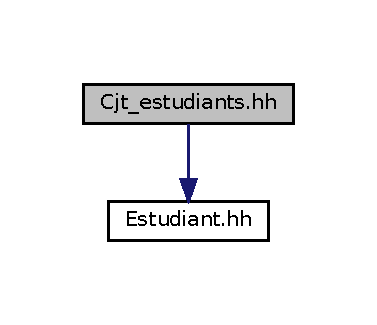
\includegraphics[width=181pt]{_cjt__estudiants_8hh__incl}
\end{center}
\end{figure}
\subsection*{Classes}
\begin{DoxyCompactItemize}
\item 
class \hyperlink{class_cjt__estudiants}{Cjt\+\_\+estudiants}
\begin{DoxyCompactList}\small\item\em Representa un conjunt d\textquotesingle{}estudiants ordenat per D\+NI. \end{DoxyCompactList}\end{DoxyCompactItemize}


\subsection{Descripció Detallada}
Especificació de la classe \hyperlink{class_cjt__estudiants}{Cjt\+\_\+estudiants}. 


\hypertarget{_estudiant_8hh}{}\section{Referència del Fitxer Estudiant.\+hh}
\label{_estudiant_8hh}\index{Estudiant.\+hh@{Estudiant.\+hh}}


Especificació de la classe \hyperlink{class_estudiant}{Estudiant}.  


\subsection*{Classes}
\begin{DoxyCompactItemize}
\item 
class \hyperlink{class_estudiant}{Estudiant}
\begin{DoxyCompactList}\small\item\em Representa un estudiant amb D\+NI i la possibilitat de tenir nota. \end{DoxyCompactList}\end{DoxyCompactItemize}


\subsection{Descripció Detallada}
Especificació de la classe \hyperlink{class_estudiant}{Estudiant}. 


\hypertarget{pro2_8cc}{}\section{Referència del Fitxer pro2.\+cc}
\label{pro2_8cc}\index{pro2.\+cc@{pro2.\+cc}}


Programa principal per l\textquotesingle{}exercici X90633.  


Inclou el graf de dependències per a pro2.\+cc\+:
\nopagebreak
\begin{figure}[H]
\begin{center}
\leavevmode
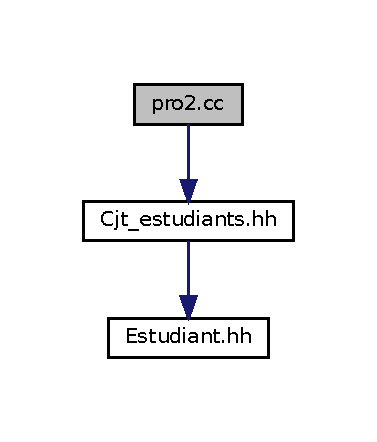
\includegraphics[width=181pt]{pro2_8cc__incl}
\end{center}
\end{figure}
\subsection*{Funcions}
\begin{DoxyCompactItemize}
\item 
int \hyperlink{pro2_8cc_ae66f6b31b5ad750f1fe042a706a4e3d4}{main} ()
\begin{DoxyCompactList}\small\item\em Programa principal per l\textquotesingle{}exercici X90633. \end{DoxyCompactList}\end{DoxyCompactItemize}


\subsection{Descripció Detallada}
Programa principal per l\textquotesingle{}exercici X90633. 



\subsection{Documentació de les Funcions}
\mbox{\Hypertarget{pro2_8cc_ae66f6b31b5ad750f1fe042a706a4e3d4}\label{pro2_8cc_ae66f6b31b5ad750f1fe042a706a4e3d4}} 
\index{pro2.\+cc@{pro2.\+cc}!main@{main}}
\index{main@{main}!pro2.\+cc@{pro2.\+cc}}
\subsubsection{\texorpdfstring{main()}{main()}}
{\footnotesize\ttfamily int main (\begin{DoxyParamCaption}{ }\end{DoxyParamCaption})}



Programa principal per l\textquotesingle{}exercici X90633. 



Definició a la línia 18 del fitxer pro2.\+cc.


\begin{DoxyCode}
18            \{
19   \hyperlink{class_cjt__estudiants}{Cjt\_estudiants} c;
20   c.\hyperlink{class_cjt__estudiants_aa24c2d4c36167b2b810ab459435b67a8}{llegir}();
21  
22   \textcolor{keywordtype}{int} op = readint();
23   \textcolor{keywordflow}{while} (op!= -5)\{
24     \hyperlink{class_estudiant}{Estudiant} est; 
25     \textcolor{keywordtype}{int} dni; 
26     \textcolor{keywordtype}{bool} b;
27     \textcolor{keywordflow}{switch} (op)\{ 
28     \textcolor{keywordflow}{case} -1:   \textcolor{comment}{// afegir estudiant}
29       est.\hyperlink{class_estudiant_af5c4883975828647dfb5ffc6735740e6}{llegir}();
30       c.\hyperlink{class_cjt__estudiants_a4188715904e017fa15b9ad8bc63112b6}{afegir\_estudiant}(est,b);
31       \textcolor{keywordflow}{if} (b)  cout << \textcolor{stringliteral}{"L'estudiant "} << est.\hyperlink{class_estudiant_ad37108e53c6c0f1fcb5786e77e1902f5}{consultar\_DNI}() << \textcolor{stringliteral}{" ja hi era"} << endl << endl;
32       \textcolor{keywordflow}{break};
33     \textcolor{keywordflow}{case} -2:   \textcolor{comment}{// esborrar estudiant}
34       cin >> dni; \textcolor{comment}{//  dni de l'estudiant a esborrar}
35       c.\hyperlink{class_cjt__estudiants_a6632e0cecaa9d698cb51da07c9e58402}{esborrar\_estudiant}(dni,b);
36       \textcolor{keywordflow}{if} (not b)  cout << \textcolor{stringliteral}{"L'estudiant amb dni "} << dni << \textcolor{stringliteral}{" no hi era"} << endl << endl;      
37      \textcolor{keywordflow}{break}; 
38     \textcolor{keywordflow}{case} -3:   \textcolor{comment}{// escriure conjunt}
39       cout << \textcolor{stringliteral}{"Conjunt:"} << endl;
40       c.\hyperlink{class_cjt__estudiants_a2c25dbd33850025de3389617712f896a}{escriure}();
41       cout << endl;
42       \textcolor{keywordflow}{break};
43     \textcolor{keywordflow}{case} -4:   \textcolor{comment}{// mitjana conjunt}
44       cout << \textcolor{stringliteral}{"Nota mitjana: "};
45       cout << c.\hyperlink{class_cjt__estudiants_a8c8099d5080864a677743e5e1d1bbdf8}{mitjana\_estudiants\_amb\_nota}() << endl << endl;
46     \}
47     op = readint();
48   \}
49 \}
\end{DoxyCode}

%--- End generated contents ---

% Index
\backmatter
\newpage
\phantomsection
\clearemptydoublepage
\addcontentsline{toc}{chapter}{Índex}
\printindex

\end{document}
